\documentclass{article}
% \usepackage{showframe}
\usepackage{siunitx}
\usepackage{booktabs}
\usepackage{graphicx}
\usepackage{amsmath}
\usepackage{mathtools}
% \usepackage{minted}
\usepackage{tabularx}
\usepackage{url}
% \usepackage{subfig}
% \usemintedstyle{xcode}

% \usepackage{fullpage}

\frenchspacing
% \setlength{\parindent}{0ex}
% \setlength{\parskip}{3 ex plus 2 ex minus 1 ex}

\title{Homework 8}
\author{Josh Bradt}
\date{April 4, 2016}

\begin{document}

\maketitle

I compiled and ran my code for the different test cases on Blue Waters using its default (Cray) compiler and MPI implementation. I requested 32 full Cray XE6 nodes using \texttt{-l nodes=32:ppn=32:xe} in my job script and ran using \texttt{aprun} with the flags \texttt{-n 32 -N 1}, which (hopefully) ran one MPI process on each node.

The results of the timing measurements are shown in Figure~\ref{fig:res}. For each test, the communications between adjacent nodes took the same amount of time (within error) regardless of which two adjacent nodes were communicating. Communication between distant nodes, on the other hand, took longer, as expected. The blocking and non-blocking ping-pong tests took the same amount of time in each case, while the head-to-head test was always faster. This is likely because in the head-to-head case, the program does not need to wait for one message to be sent before sending the second one.

\begin{figure}
    \centering
    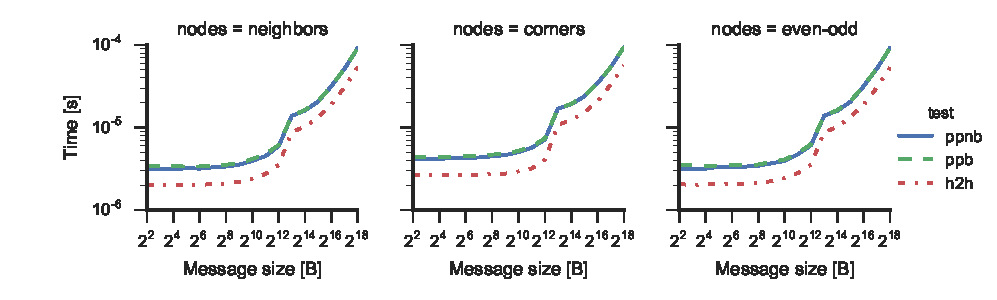
\includegraphics[width=\textwidth]{databynodes.pdf}
    \caption{Measured time for each test case. Each column represents a different set of nodes. In these cases, ``neighbors'' means nodes 0 and 1, ``corners'' means nodes 0 and 31, and ``even-odd'' means nodes 2 and 3. Each color / line style represents a different test case. Here, ``ppnb'' means ping-pong with non-blocking MPI send/receive, ``ppb'' means ping-pong with blocking communications, and ``h2h'' means the head-to-head communication case with non-blocking calls.}
    \label{fig:res}
\end{figure}

The results of a linear fit to the blocking ping-pong test between nodes 0 and 1 are shown in Figure~\ref{fig:fitres}, and the parameters of these fits are listed in Table~\ref{tab:fit}.

\begin{figure}
    \centering
    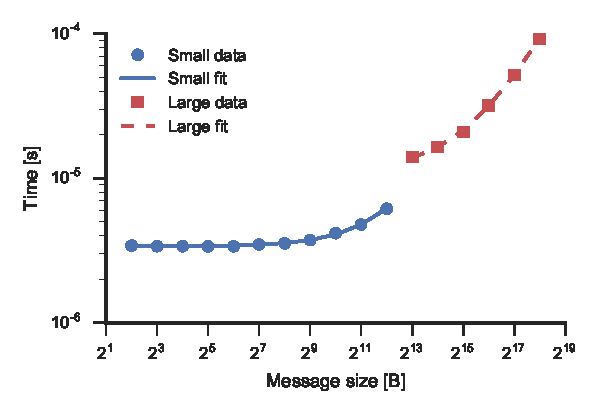
\includegraphics{fitresults.pdf}
    \caption{Results of a linear fit to the blocking ping-pong test between nodes 0 and 1. Note that the curves appear to be non-linear because of the log-log scale. The data had to be broken into two sets due to the discontinuity between 4096 and 8192 bytes. The parameters of these fits are shown in Table~\ref{tab:fit}.}
    \label{fig:fitres}
\end{figure}

\begin{table}
    \centering
    \begin{tabular}{cS[table-format=1.3e+2]S[table-format=1.3e+3]}
        \toprule
        {Group} & {$s\ [\si{s}]$}     & {$r\ [\si{s/B}]$} \\ \midrule
        Small   & 3.384e-06      & 6.814e-10    \\
        Large   & 1.128e-05      & 3.100e-10    \\
        \bottomrule
    \end{tabular}
    \caption{Fit parameters for the two fits shown in Figure~\ref{fig:fitres}. The ``Small'' group contains data from \SIrange{4}{4096}{B}, and the ``Large'' group contains the data from \SIrange{8192}{262144}{B}. The fitted model was $t(n) = s + rn$.}
    \label{tab:fit}
\end{table}

\end{document}
